% -----------------------------------------------------------------------
% -----------------------------------------------------------------------
\section*{Backpropagation Through Time (BPTT)}
Um Rekurrente Neuronale Netze (RNNs) zu trainieren gibt es mehrere Möglichkeiten. Eine der am meist verbreiteten Methoden ist \emph{Backpropagation Through Time} (BPTT).
Dabei wird das RNN in ein feed-forward Netz (FFNN) transformiert, wofür das RNN zuerst zeitlich Entfaltet (engl. unfolding in time) und anschließend mittels Backpropagation Through Time (BPTT) trainiert wird.

\subsection*{Unfolding in Time}
Nach Minsky und Papert gibt es zu jedem RNN mit diskreten Zeitschritten für eine fest vorgegebene Zeitdauer ein äquivalentes FFNN, das dieses simulieren kann.
Allerdings hat dieses FFNN extrem viele Knoten und Verbindungen. Deshalb wird dies im Folgenden am Beispiel eines kleinen rekurrenten Netzes veranschaulicht, das in Abbildung \ref{fig:ch05_einfaches-rnn} dargestellt ist.

\begin{figure}[ht!] \centering 
	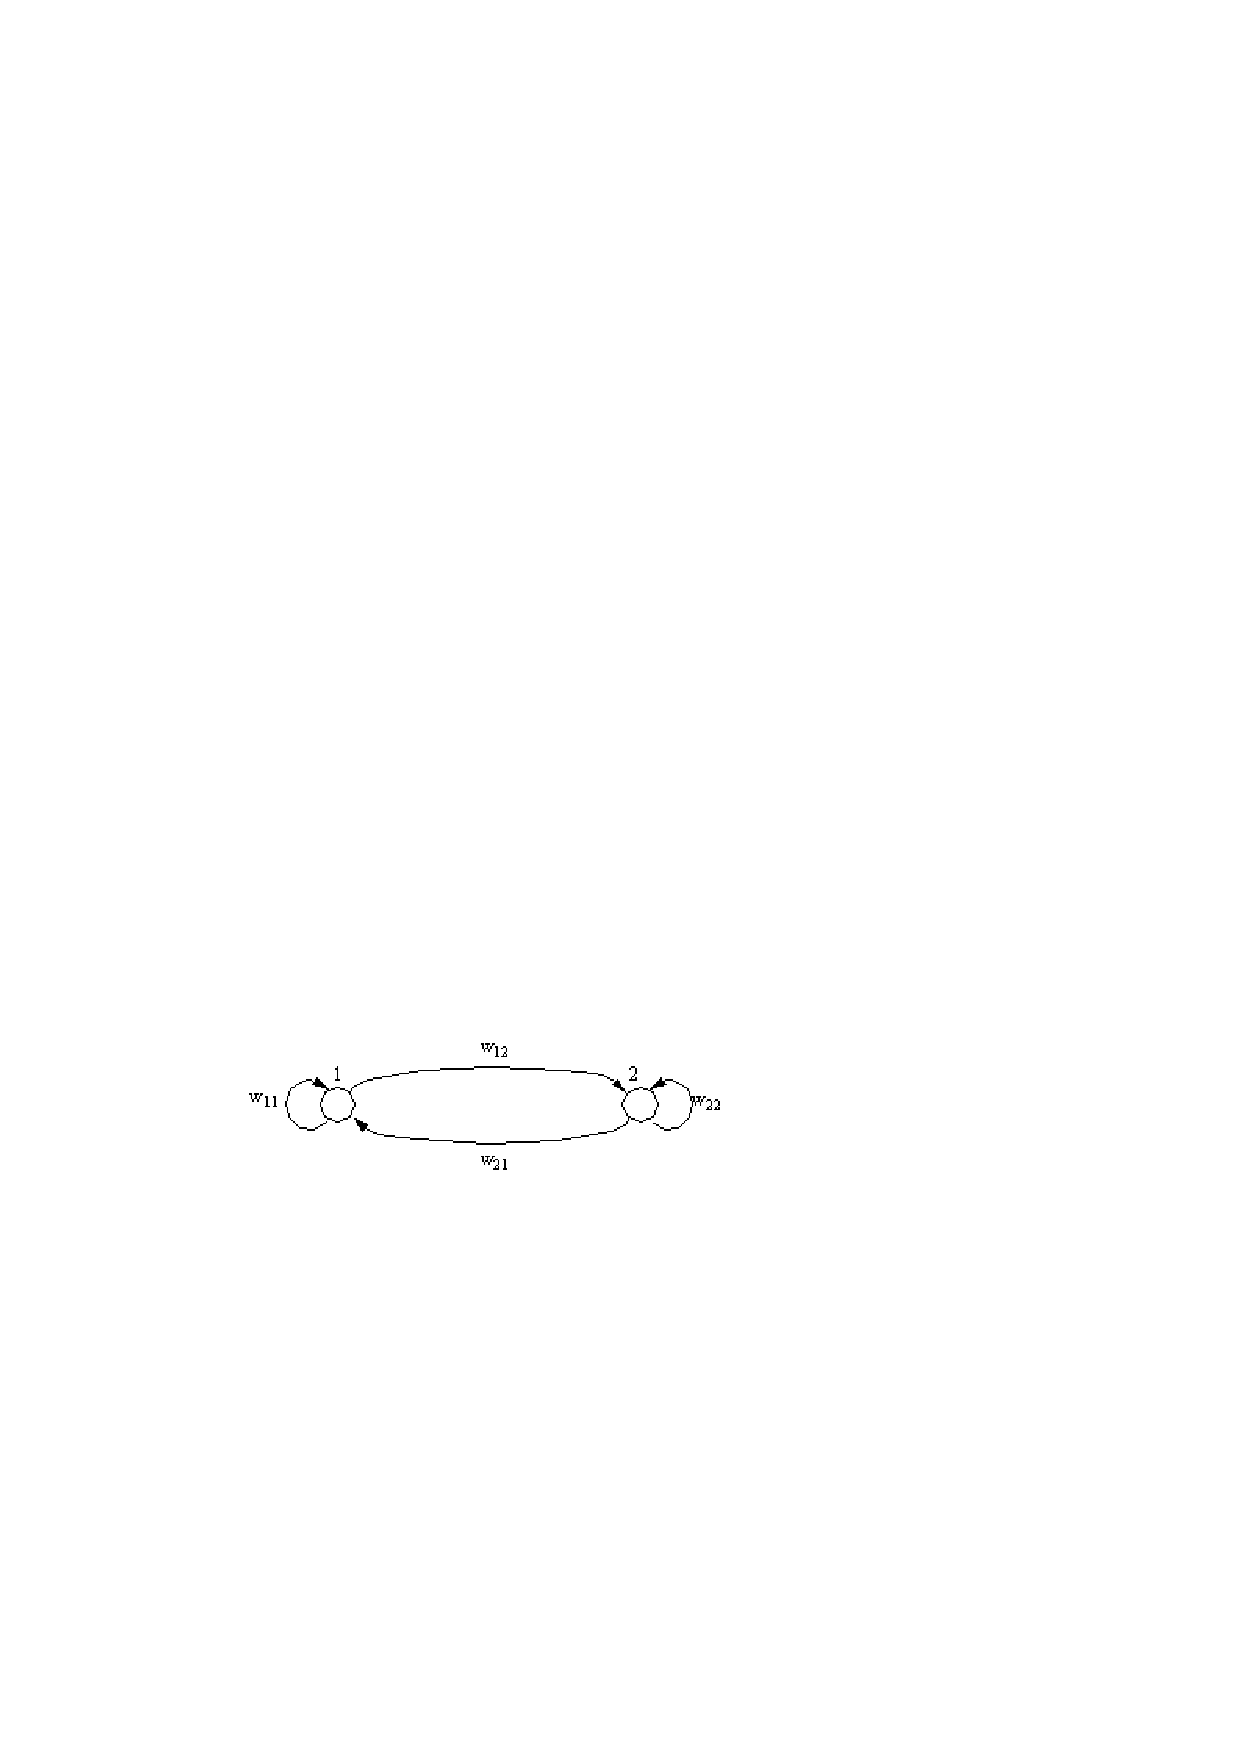
\includegraphics[width=\linewidth]{figures/ch05_einfaches-rnn.pdf}
	\caption{Einfaches RNN mit zwei Zellen.}
	\label{fig:ch05_einfaches-rnn}
\end{figure}

Durch zeitliches Entfalten werden für ein äquivalentes FFNN alle Neuronen und Gewichte des RNN für jeden diskreten Zeitschritt durch eigene Neuronen und Gewichte ersetzt. 
Dazu muss die maximale Zahl der Zeitschritte, die man untersuchen will, vorher bekannt sein. Die Verbindungsgewichte $w_{ij}$ werden dann immer von Neuron $i$ zum Zeitpunkt $t$ zu Neuron $j$ zum Zeitpunkt $t+1$ gezogen. Diese Gewichte müssen auf allen Ebenen gleich sein und den Gewichten des rekurrenten Systems entsprechen.

\begin{figure}[ht!] \centering 
	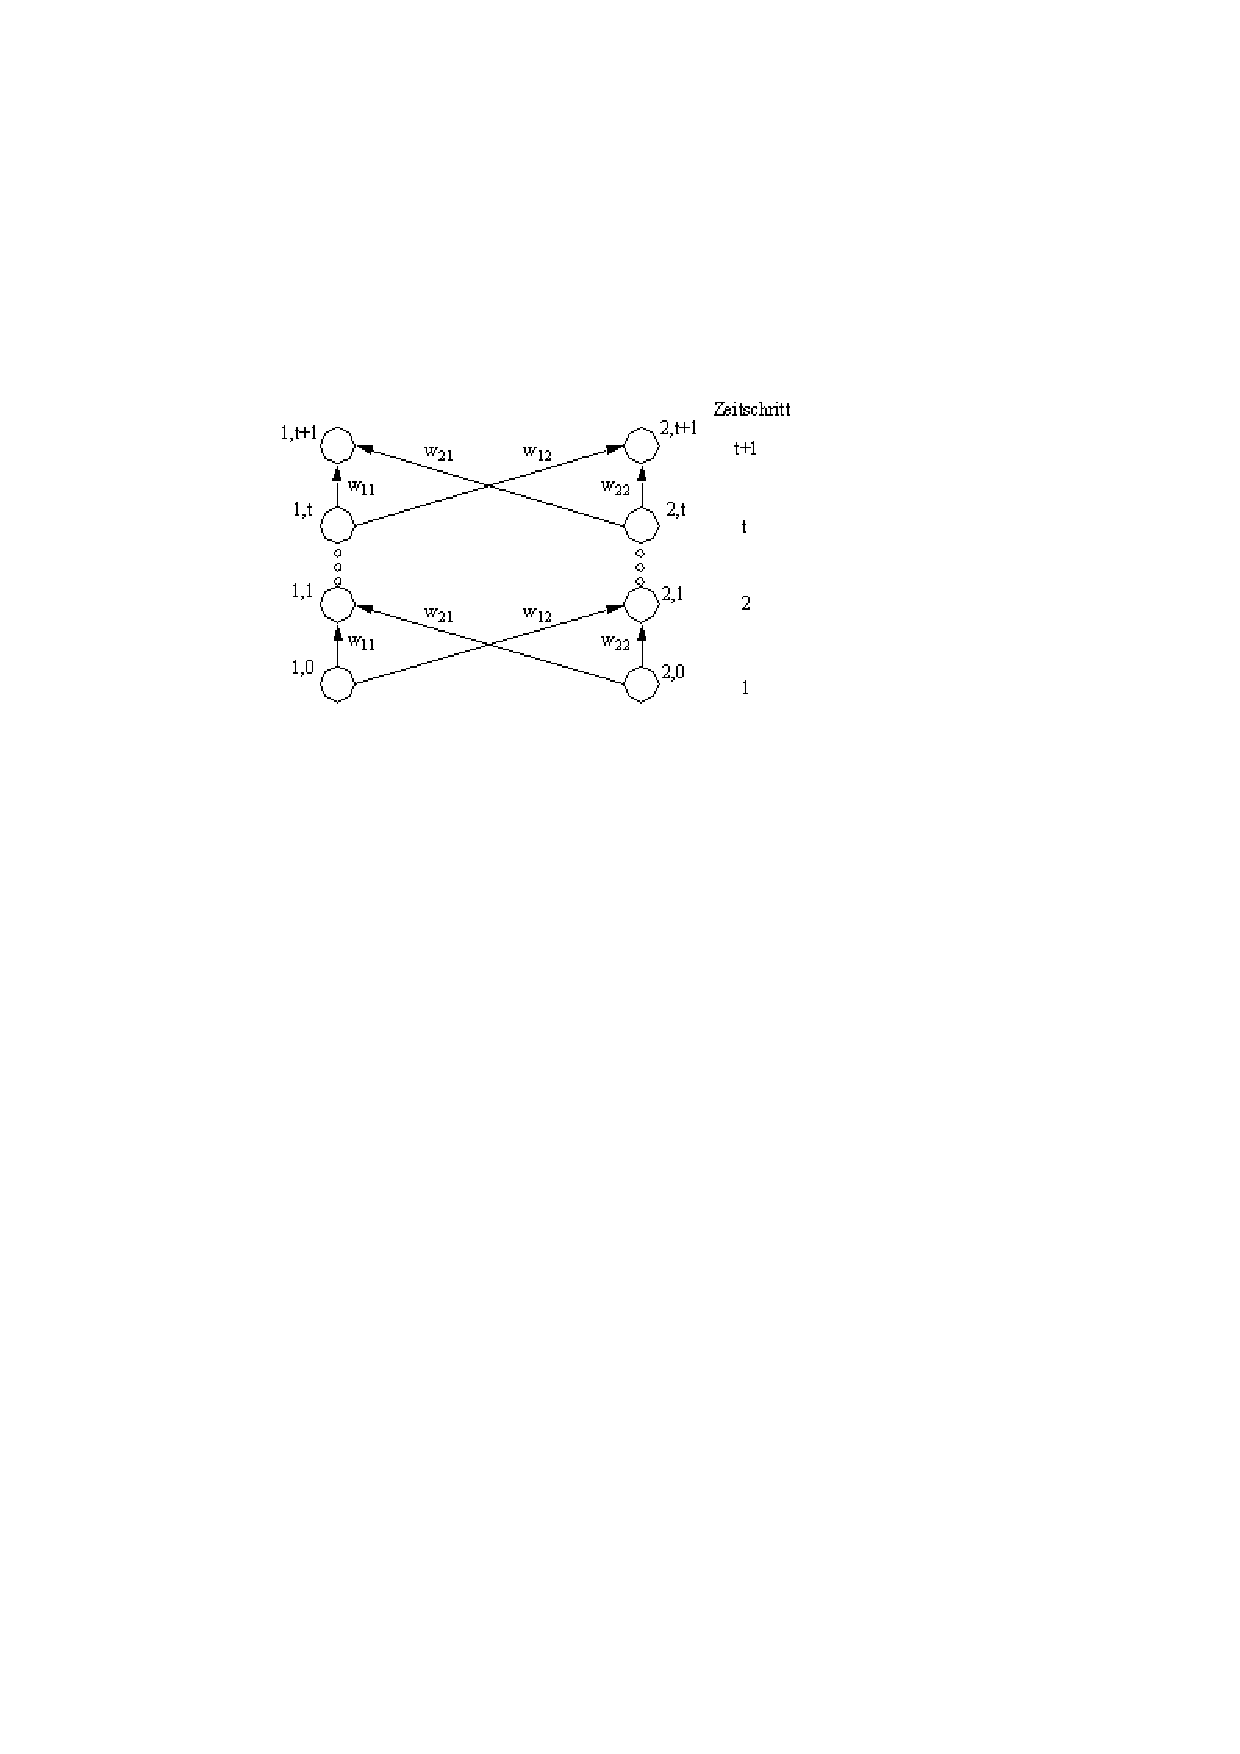
\includegraphics[width=\linewidth]{figures/ch05_ffnn-eines-rnn.pdf}
	\caption{Das zu Abbildung \ref{fig:ch05_einfaches-rnn} äquivalente FFNN.}
	\label{fig:ch05_ffnn-eines-rnn}
\end{figure}

Man sieht sofort, dass das FFNN in den Neuronen mit zweitem Index $t$ genau den Zustand anzeigt, in dem das RNN nach $t$ Zeitschritten ist. Wichtig ist hier, dass \emph{alle Gewichte mit gleichen Indizes über alle Zeitpunkte den gleichen Wert haben} (da sie ja im RNN nur als ein Gewicht vorhanden sind). Sie müssen also auch durch ein Lernverfahren alle um den gleichen Betrag geändert werden.
Mit dieser Einschränkung lässt sich dann das normale Backpropagation-Verfahren für das resultierende FFNN verwenden.

\subsection*{Weight Sharing}
Das Problem dieser Transformation ist in erster Linie der extrem hohe Speicherplatzbedarf von $O(t_{max} n^2)$ bei $n$ Neuronen und maximaler Zeitdauer $t_{max}$.

Effizienter ist eine als \emph{weight sharing} bekannte Technik, bei der die Gewichte nicht physisch vorhanden sind, sondern jeweils nur als Zeiger auf den gleichen Speicherplatz für das Gewicht. Da die Gewichte über alle Zeitschritte gleich bleiben müssen und erst nach Fehlerrückpropagierung über alle Zeitschritte um die Summe aller Änderungen geändert werden dürfen, kann man das ursprüngliche RNN, bei dem jedes Gewicht nur einmal repräsentiert war, beibehalten und sich nur die Ausgaben der Neuronen über die Zeit in einem Stapel für jedes Neuron merken. 
Dies ist in Abbildung \ref{fig:ch05_rnn-weight-sharing} dargestellt.

\begin{figure}[ht!] \centering 
	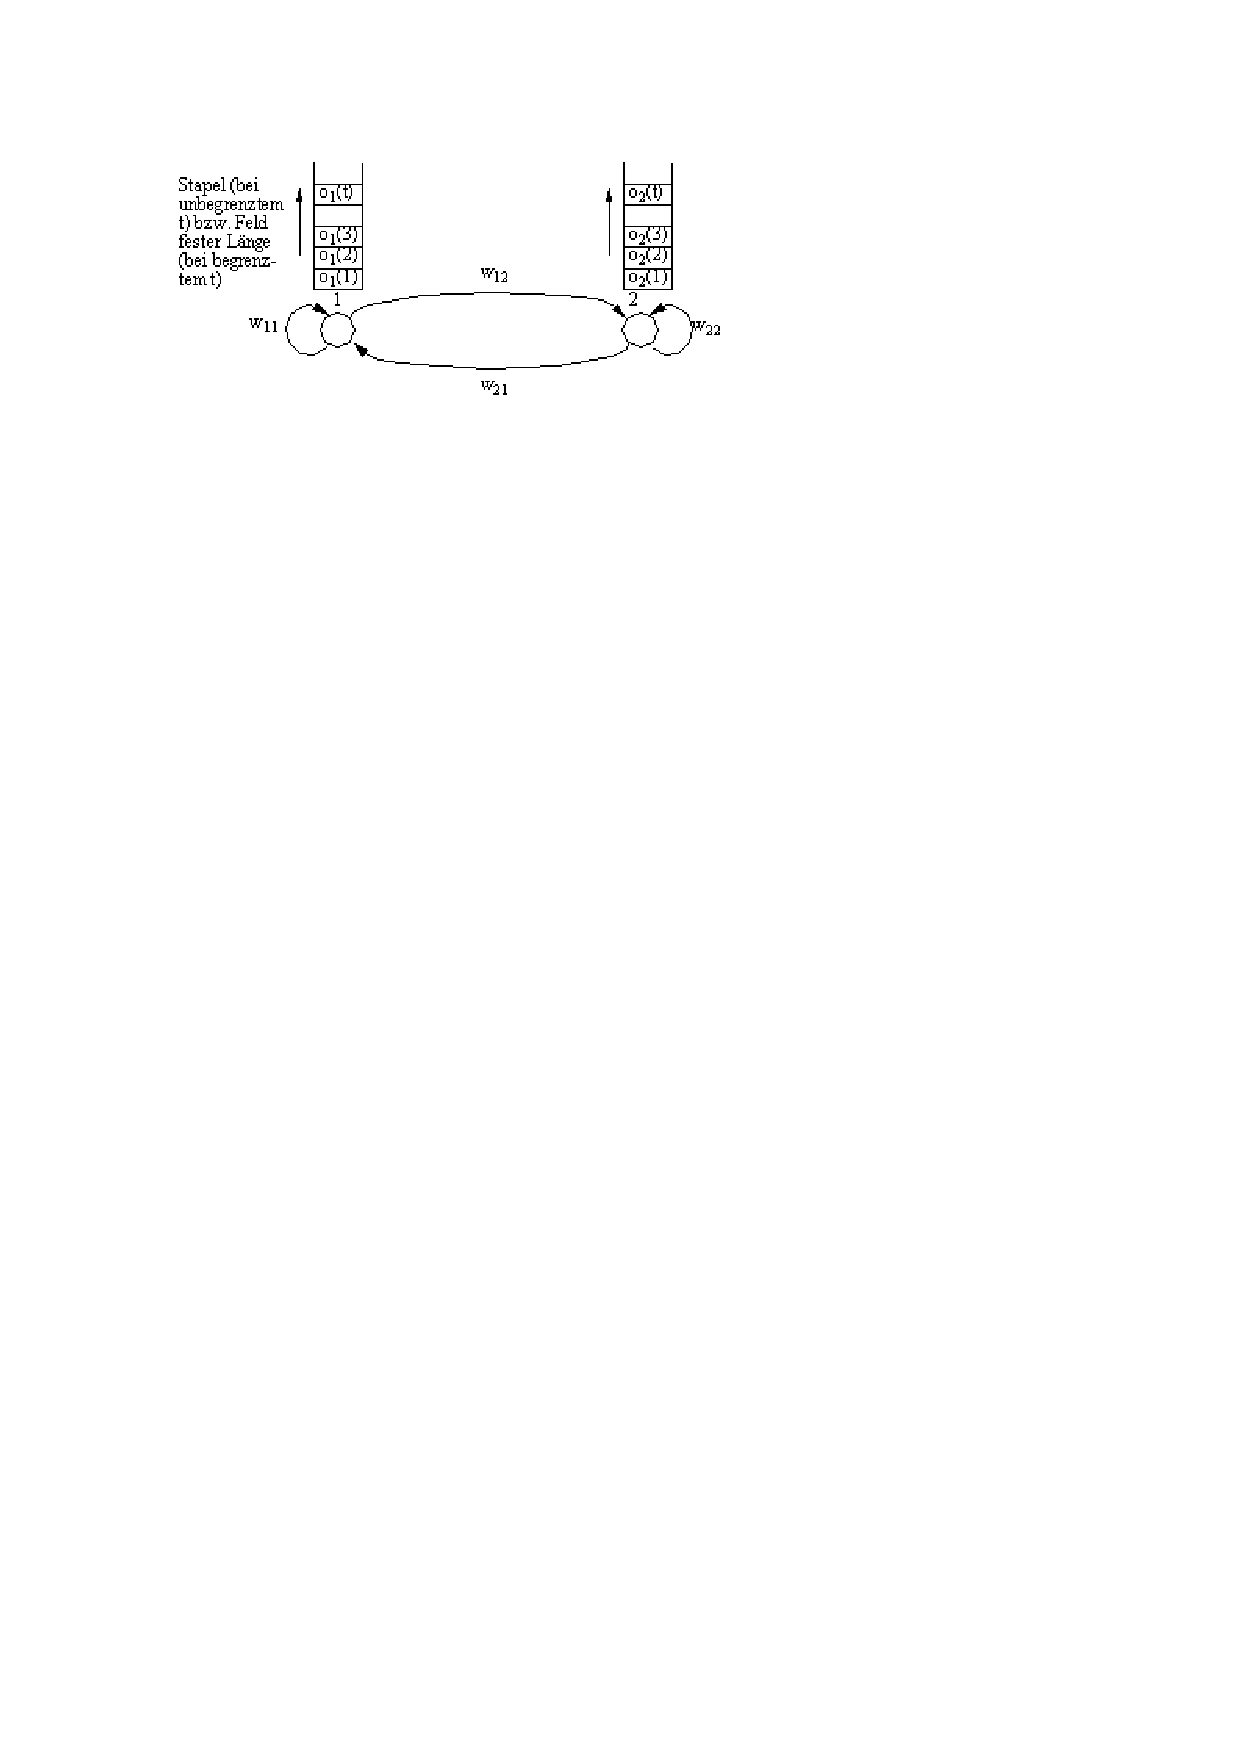
\includegraphics[width=\linewidth]{figures/ch05_rnn-weight-sharing.pdf}
	\caption{Rekurrentes Netzwerk für BPTT. Jedes Neuron besitzt einen Stapel der Ausgaben zu allen Zeitpunkten.}
	\label{fig:ch05_rnn-weight-sharing}
\end{figure}

Diese Stapel enthalten alle Ausgaben der Neuronen bis zum Zeitpunkt $t$. Neue Ausgaben werden jeweils oben auf den Stapel gelegt und nach Verwendung zur Berechnung der $\delta$-Werte für die Rückpropagierung von oben wieder gelöscht.
Da die Gewichte immer gleich bleiben sollen, brauchen sie durch weight sharing nur einmal gespeichert werden.


\subsection*{Backpropagation}
Bei rekurrenten Netzen wird üblicherweise die Eingabe (meist in Folge) angelegt, und man lässt das Netz eine Anzahl von Zyklen laufen. Zu einer bestimmten Zeit wird die Ausgabe des Netzes mit der Zielausgabe verglichen und die Fehlersignale werden für alle Ausgabeneuronen erzeugt.
Diese Fehlersignale werden dann für die gleiche Anzahl von Zyklen durch das Netz zurück propagiert. Für jede Iteration werden die Gewichtsänderungen berechnet und die Summe der Änderungen werden für jedes Gewicht gespeichert. Danach werden alle Gewichte um diese Summe geändert.

Für den Gesamtfehler $Err_p$ aller Ausgabeneuronen $k$ über die Zeit von $t=1$ bis $t=t_{max}$ gilt\footnote{In der folgenden Beschreibung wird zur besseren Übersichtlichkeit der Index $p$ für das aktuelle Muster weggelassen, die Summation über alle Muster $p$ wird an den dazu notwendigen Stellen implizit angenommen.}:
\begin{align*}
	Err_p &= \sum_{t=1}^{t_{max}} E(t)
		= \sum_{t=1}^{t_{max}} \sum_k ( E_k(t))^2 \\
	&\text{mit}\\
	E_k(t) &=
	\begin{cases}
		t_k(t) - o_k(t) &\text{falls für } k \text{ zum Zeitpunkt } t \\
			&\text{eine Ausgabe spezifiziert wurde} \\
		0	&\text{sonst}
	\end{cases}
\end{align*}
\noindent
Darüber hinaus gelten für die Gewichtsänderung $\Delta w_{ij}$ und die Fehlersignale $\delta_j$ die Zusammenhänge, welche auch beim normalen Backpropagation Algorithmus gelten:
\[
	\Delta w_{ij} = - \eta \frac{\partial E}{\partial w_{ij}}
	\quad \text{und} \quad
	\delta_j(t) = - \frac{\partial E}{\partial net_j(t)}
\]
\noindent
Für die Fehlersignale $\delta_j(t)$ gilt damit:
\begin{align*}
	\delta_j(t) = 
	\begin{cases}
		f'_{act}(net_j(t)) \cdot E_j(t) &\text{falls } t = t_{max} \\
		f'_{act}(net_j(t)) \big [ 
			E_j(t) + &\\
			\quad \sum_k \delta_k(t+1) \cdot w_{jk} \big ]
			&\text{falls } 1 \le t \le t_{max}
	\end{cases}
\end{align*}

\noindent
Daraus ergibt sich folgende Formel für die Gewichtsänderung nach Präsentation eines Musters über die gesamte Zeitdauer von $t=1$ bis $t=t_{max}$:
\[
	\Delta w_{ij} = - \eta \frac{\partial E}{\partial w_{ij}} =
		\eta \sum_{t=1}^{t_{max}} \delta_j(t) \cdot o_i(t-1)
\]

Die \emph{Zeitkomplexität} dieses Algorithmus beträgt für jeden Durchgang durch alle Zeitschritte $O(t_{max} n^2)$.

Der \emph{Speicherplatzbedarf} beträgt in dieser Realisierung nur noch $O(t_{max} n + n^2)$.

\subsection*{Fazit}
Backpropagation Through Time ist ein sehr effizientes Verfahren zum Training beliebiger rekurrenter Netze, wenn die Länge der zeitlichen Muster kleiner oder gleich der Anzahl der Neuronen des Netzwerks ist.

Für sehr lange Eingabesequenzen sind andere Verfahren, beispielsweise Real-Time Recurrent Learning (RTRL) oder die Kombination von BPTT mit RTRL von Schmidhuber besser geeignet.


% -----------------------------------------------------------------------
% -----------------------------------------------------------------------
\section*{Real-Time Recurrent Learning (RTRL)}
Real-Time Recurrent Learning ist eine Variante von Backpropagation für rekurrente Netze, die von Williams und Zipser vorgeschlagen wurde. Es verwendet die gleiche Vorwärtsdynamik wie Backpropagation Through Time.

Die eigentlich interessante Version dieses Verfahrens ist die \emph{online}-Version, bei der die Gewichte nach jedem Zeitschritt geändert werden:
\[
	w_{ij}(t+1) = w_{ij}(t) + \Delta w_{ij}(t)
\]
In diesem Fall werden die Gewichtsänderungen schon durchgeführt, während das Netzwerk sich noch nicht über die volle Zeitsequenz angepasst hat. Dies hat den großen Vorteil, dass keine Begrenzung der Trainingssequenz mehr notwendig ist und keine Epochengrenzen des Trainings mehr eingehalten werden müssen. 
Es ist also ein online-Lernen in "`Echtzeit"' möglich, was zur Namensgebung Real-Time Recurrent Learning geführt hat.

\begin{hint}{Hinweis!}{rtrl}
	Das RTRL-Verfahren wurde in der Vorlesung \emph{nicht} behandelt und ist nur aus Gründen der Vollständigkeit und in stark verkürzter Form hier aufgeführt.
\end{hint}

% -----------------------------------------------------------------------
% -----------------------------------------------------------------------
\section*{Kombination von BPTT und RTRL}
Von J. Schmidhuber stammt ein Verfahren, das durch eine Kombination von BPTT und RTRL eine Beschleunigung der Zeitkomplexität von RTRL um den Faktor $n$ (der Anzahl der Neuronen im rekurrenten Netzwerk) erreicht.
Alle $n$ Zeitschritte benötigt das hybride Verfahren $O(n^4)$ Operationen, bei den $n$ dazwischenliegenden Zeitschritten dagegen nur jeweils $O(n^2)$ Operationen. Das entspricht einer durchschnittlichen Zeitkomplexität von $O(n^3)$ Operationen pro Zeitschritt.

Auch bei diesem Algorithmus kann man eine offline-Version und eine online- Version unterscheiden: Die offline-Version führt die Gesamtgewichtsänderung nach Abschluss der Präsentation aller Trainingssequenzen aus.
Die entsprechende online-Version ändert die Gewichte jeweils nach dem vierten Schritt, also jeweils nach Abarbeitung eines Blocks der Zeitdauer $n$.

In verschiedenen Experimenten mit (in erster Linie theoretisch interessanten) Benchmark-Netzen konnte Schmidhuber zeigen, dass seine hybride Methode dem Verfahren RTRL deutlich überlegen war.
Er empfiehlt aber selbst die Verwendung von RTLR oder des hybriden Verfahrens nur dann, wenn die Länge der Trainingssequenzen sehr lang im Verhältnis zu Anzahl der Knoten des Netzwerks ist. 
Ist diese Länge kleiner als $n$, dann ist BPTT das bessere Verfahren.

\begin{hint}{Hinweis!}{rtrl}
	Die Kombination von BPTT und RTRL wurde in der Vorlesung \emph{nicht} behandelt und ist nur aus Gründen der Vollständigkeit und in stark verkürzter Form hier aufgeführt.
\end{hint}


% -----------------------------------------------------------------------
% -----------------------------------------------------------------------
\section*{Rekurrentes Backpropagation}
Darüber hinaus existiert ein Verfahren für Backpropagation für beliebige rekurrente Netze \emph{ohne Zeitbeschränkung}.

Dieses wurde als Zeitabhängige rekurrente Backpropagation (engl. Time-Dependent Recurrent Backpropagation) mit kontinuierlicher Zeit verallgemeinert. Dies ist insbesondere für analoge Realisierungen rekurrenter Backpropagation-Netze und diskrete Simulationen auf Digitalrechnern interessant.

Der Unterschied zwischen rekurrentem Backpropagation und zeitabhängigem rekurrentem Backpropagation liegt darin, dass man bei ersterem annimmt, dass ein stabiler Attraktor existiert, und diesen vom gegebenen Zustand zu finden sucht, während man bei letzterem eine Trajektorie trainiert, die sich auch über Grenzzyklen hinweg zu einem Attraktor bewegen kann. 

\begin{hint}{Hinweis!}{rtrl}
	Auch diese beiden Themen wurde in der Vorlesung \emph{nicht} behandelt und sind nur aus Gründen der Vollständigkeit und in stark verkürzter Form hier aufgeführt.
\end{hint}